%%%%%%%%%%%%%%%%%%%%%%%%%%%%%%%%%%%%%%%%%%%%%%%%%%%%%%%%%%%%%%%%%%%%%%%%%%%%%%%
%
% Introduction
% 
%%%%%%%%%%%%%%%%%%%%%%%%%%%%%%%%%%%%%%%%%%%%%%%%%%%%%%%%%%%%%%%%%%%%%%%%%%%%%%%


\chapter{Introduction}
Fluid-Structure Interaction (FSI) problems describe the coupled dynamics of fluid mechanics and structure mechanics. They are classical multi-physics problems and its application is very vast. Numerical simulation of such problems is a cumbersome process. There are mainly two approaches in solving the FSI problems \textit{Monolithic approach} and \textit{Partitioned approach}. In the current study, the focus is on the partitioned approach for solving FSI problems. Partitioned analysis techniques are more popular than the fully coupled Monolithic solvers, as they have computational superiority over the Monolithic solvers. Partitioned solvers allows for the use of suitable discretization methods, and optimized solvers for modeling of both fluid and structure. In the current investigation, adaptive schemes such as \textit{Aitken's $\Delta^2$ method} and \textit{Steepest descent/gradient method} are implemented into the FSI solver to predict the \textit{under-relaxation factor} dynamically. The current study also involves integration of an \textit{Artificial Neural Network (ANN)} within the FSI solver for dynamic prediction of under-relaxation factors. The calculations are performed on an in-house \textit{finite volume} based \textit{FORTRAN} solver, \textit{FASTEST-3D}. A partitioned, semi-implicit predictor-corrector coupling scheme method is used for solving FSI problems. 

\section{Need for dynamic relaxation methods}
Partitioned schemes uses two separate solvers for solving fluid and structural equations. Strongly coupled methods require several sub-iterations for a particular time-step. And by their nature, iterative solvers require a convergence criteria which determines the termination of the iterations. In order to aid the convergence of the iterative solvers, relaxation factors are used. They can either be over-relaxation or under-relaxation parameters, in this study the focus is on under-relaxation factors $\omega \in \left(0,1\right)$.
 
The most basic and easiest implementation is to use a \textit{constant under-relaxation} factor for every iteration. This is not the most effective method, but it is robust and easy to implement. However, a poorly chosen under-relaxation factor can lead to numerical instabilities and ultimately slow down convergence. This leads to higher computational time and effort. There are no universal guidelines for selecting an appropriate constant under-relaxation factor, because they depend not only on the physical processes being approximated, but also on the details of the numerical formulation. It is often selected based on trial-and-error method for each problem.

In order to alleviate the problem, several adaptive methods can be found in literature for performing sub-iterations in an efficient and robust fashion. \citet{mok2001partitioned}, \citet{wall1999partitioned} proposed the most basic and highly efficient approach, the fixed-point iteration method with
dynamic relaxation. \citet{wall1999partitioned} compared the effectiveness of three different methods, the \textit{Aitken relaxation method}, \textit{Tschebyscheff relaxation method} and \textit{the method of steepest descent}. However, this work is only available in two hardly available conference proceedings and was never published in any journal.

\citet{kuttler2008fixed} reproduced the work of \citet{mok2001partitioned},and \citet{wall1999partitioned} where the treatment of both the \textit{Aitken relaxation method} and \textit{relaxation via the method of steepest descent} in the context of fixed-point iteration FSI solvers are studied. As per their study, the main advantage of fixed-point FSI solvers based on a Dirichlet–Neumann partitioning is the simple implementation with available field solvers. The calculation of a specific relaxation parameter in each iteration step influenced the convergence criteria. The relaxation methods were extended to FSI solvers based on Newton-Krylov methods. The Aitken relaxation method, proposed by \citet{irons1969version} was found to be the most simple yet efficient method. \citet{yigit2007efficiency} investigated the efficiency of acceleration techniques for fluid structure interaction computations. The computations were carried out on a finite volume flow solver \textit{FASTEST}, which is the solver used for the current study. \citet{yigit2007efficiency} implemented a multigrid procedure for moving meshes together with an adaptive under-relaxation strategy for accelerating the coupled computations. An Aitken relaxation method was integrated into the multigrid solver and the acceleration of the convergence were studied. The acceleration of the convergence improved with the integration of an adaptive under-relaxation technique. 

\citet{valdes2016nonlinear} implemented an algorithm to analyze the structures with large deformations, incompressible fluid flows and its fluid-structure interaction problems. This study emphasizes the use of \textit{block-Gauss-Seidel method} with relaxation techniques.       It has been observed that the strong coupling block Gauss-Seidel partition method with a relaxation method based on Aitken's method provided accelerated convergence for a variety of problems. \citet{bogaers2014quasi} implemented a \textit{Quasi-Newton method} with adaptive under-relaxation technique for implicit coupling of FSI solvers. It has been observed that for higher added mass ratios, the quasi-Newton methods with dynamic relaxation provides better results, when compared to fixed point iteration technique with dynamic relaxation.    

\section{Thesis objective}
In the current study, the dynamic relaxation methods \textbf{Aitken's relaxation method} and \textbf{Steepest-Descent method} are implemented. The implementation is carried out on an in-house finite volume solver \textbf{FASTEST-3D}, a FORTRAN based solver. The coupling of the fluid and structure solver is done via a \textit{semi-implicit predictor-corrector coupling}. Owing to the effectiveness and ease of implementation, these dynamic relaxation methods are selected and implemented. The FSI simulation of vortex induced vibration of a cylinder is validated and the effectiveness of the adaptive schemes is studied. The study replicates the work of \citet{zhou1999vortex}, and the results of the simulation are compared and validated. The setup replicates the spring mass damper system, as represented in the figure \ref{fig:1.1}. 

\begin{figure}[h]
\centering
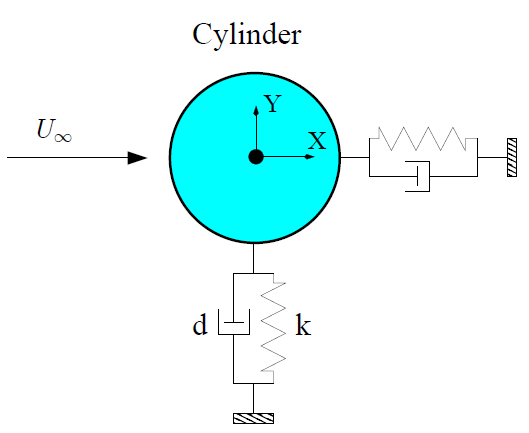
\includegraphics[height=3in]{smd}
\caption{Representation of a spring-mass-damper system}
\label{fig:1.1}
\end{figure} 

The dynamic relaxation factors are then trained on a \textit{Tensorflow MLP Regressor} neural network model. The trained model is then integrated externally via a shell script into the FASTEST-3D solver to predict the under-relaxation factors dynamically. The acceleration properties are studied and compared for these dynamic methods. 

The thesis is structured as follows: An overview into the theoretical background related to the task is presented in the chapter 2. Chapter 3 discusses the numerical treatment of the methods used. The results from these methods are validated and presented in detail in chapter 4. Conclusive remarks are presented in chapter 5.  
